\setmodule{9}

%BEGIN_FOLD % ====>>_____ Занятие 1 _____<<====
\begin{class}[number=1]
	\begin{listofex}
		%255-257
		\item На рисунке представлены графики линейных функций. Для каждой функции определите знаки \(k\) и \(b\). \\
		\begin{minipage}[t]{0.45\linewidth}
			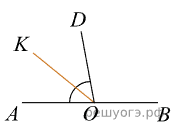
\includegraphics[align=t, width=\linewidth]{\picpath/../../bank/graphs/graph_gleb/7/1}
		\end{minipage}
		\gapwidth
		\begin{minipage}[t]{0.45\linewidth}
			\includegraphics[align=t, width=\linewidth]{\picpath/../../bank/graphs/graph_gleb/7/2}
		\end{minipage}
		\item 
		\begin{minipage}[t]{\bodywidth}
			Сопоставьте каждому уравнению его график:
			\begin{tasks}
				\task \( y=-2x+5 \)
				\task \( y=-\dfrac{ 2 }{ 3 }x+5 \)
				\task \( y=-6x+5 \)
			\end{tasks}
		\end{minipage}
		\gapwidth
		\begin{minipage}[t]{\picwidth}
			\includegraphics[align=t, width=\linewidth]{\picpath/../../bank/graphs/graph_gleb/7/3}
		\end{minipage}
		\item 
		\begin{minipage}[t]{\bodywidth}
			Сопоставьте каждому уравнению его график:
			\begin{tasks}
				\task \( y=-2x+5 \)
				\task \( y=-2x \)
				\task \( y=-2x-5 \)
			\end{tasks}
		\end{minipage}
		\gapwidth
		\begin{minipage}[t]{\picwidth}
			\includegraphics[align=t, width=\linewidth]{\picpath/../../bank/graphs/graph_gleb/7/4}
		\end{minipage}
		%260 а-г
		\item Не выполняя построения, определите, в каких четвертях лежит график
		функции:
		\begin{tasks}(2)
			\task \( y=9x-6 \)
			\task \( y=-8 \)
			\task \( y=-5x \)
			\task \( y=-2x+7 \)
		\end{tasks}
		\item По озеру плавала яхта. Расстояние \(s\) (в километрах), на которое удалялась яхта от базы, менялось с течением времени движения (в минутах). Изменение \(s\) в зависимости от t показано на рисунке. 
		\begin{tasks}
			\task На каком расстоянии от базы находилась яхта через \(20\) минут?
			\task На каком расстоянии от базы находилась яхта через \(1\) час \(20\) минут?
			\task На каком расстоянии от базы находилась яхта через \(2\) часа \(30\) минут?
			\task Какова область определения рассматриваемой функции?
		\end{tasks}
		\begin{minipage}[t]{\linewidth}
			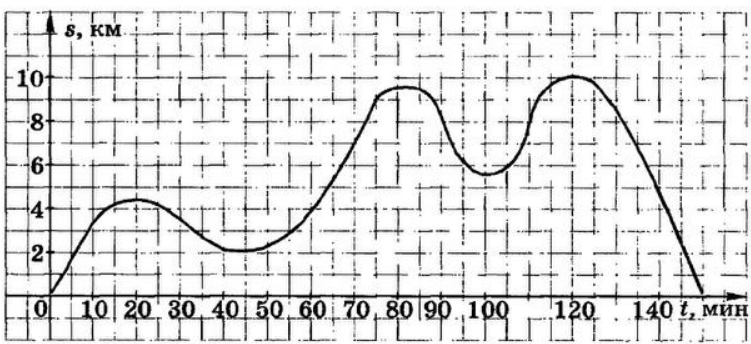
\includegraphics[align=t, width=\linewidth]{\picpath/../../bank/graphs/graph_gleb/7/G71M9L1-1}
		\end{minipage}
		\item Функция задана формулой \(y=\dfrac{ 12 }{ x }\). В таблице указаны некоторые значения аргумента. Заполните таблицу, вычислив соответствующие значения функции:
		\begin{minipage}[t]{\linewidth}
			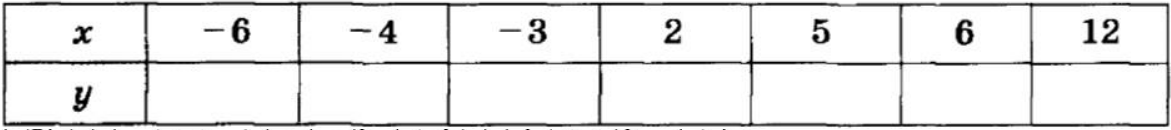
\includegraphics[align=t, width=\linewidth]{\picpath/../../bank/graphs/graph_gleb/7/G71M9L1-2}
		\end{minipage}
		\item Функция задана формулой \(y=\dfrac{ 2}{ 3 }x\). Заполните таблицу:
		\begin{minipage}[t]{\linewidth}
			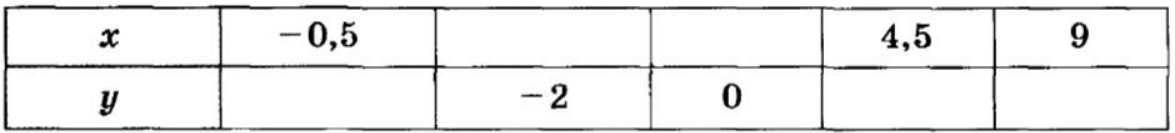
\includegraphics[align=t, width=\linewidth]{\picpath/../../bank/graphs/graph_gleb/7/G71M9L1-3}
		\end{minipage}
	\end{listofex}
\end{class}
%END_FOLD

%BEGIN_FOLD % ====>>_____ Занятие 2 _____<<====
\begin{class}[number=2]
	\begin{listofex}
		\item Занятие 2
	\end{listofex}
\end{class}
%END_FOLD

%BEGIN_FOLD % ====>>_ Домашняя работа 1 _<<====
\begin{homework}[number=1]
	\begin{listofex}
		\item Домашняя работа 1
	\end{listofex}
\end{homework}
%END_FOLD

%BEGIN_FOLD % ====>>_____ Занятие 3 _____<<====
\begin{class}[number=3]
	\begin{listofex}
		\item Занятие 3 
	\end{listofex}
\end{class}
%END_FOLD

%BEGIN_FOLD % ====>>_____ Занятие 4 _____<<====
\begin{class}[number=4]
	\begin{listofex}
		\item Занятие 4
	\end{listofex}
\end{class}
%END_FOLD

%BEGIN_FOLD % ====>>_ Домашняя работа 2 _<<====
\begin{homework}[number=2]
	\begin{listofex}
		\item Домашняя работа 2
	\end{listofex}
\end{homework}
%END_FOLD

%BEGIN_FOLD % ====>>_____ Занятие 5 _____<<====
\begin{class}[number=5]
	\begin{listofex}
		\item Занятие 5
	\end{listofex}
\end{class}
%END_FOLD

%BEGIN_FOLD % ====>>_____ Занятие 6 _____<<====
\begin{class}[number=6]
	\begin{listofex}
		\item Занятие 6
	\end{listofex}
\end{class}
%END_FOLD

%BEGIN_FOLD % ====>>_ Домашняя работа 3 _<<====
\begin{homework}[number=3]
	\begin{listofex}
		\item Домашняя работа 3
	\end{listofex}
\end{homework}
%END_FOLD

%BEGIN_FOLD % ====>>_____ Занятие 7 _____<<====
\begin{class}[number=7]
	\title{Подготовка к проверочной}
	\begin{listofex}
		\item Занятие 7
	\end{listofex}
\end{class}
%END_FOLD

%BEGIN_FOLD % ====>>_ Проверочная работа _<<====
\begin{exam}
	\begin{listofex}
		\item Проверочная
	\end{listofex}
\end{exam}
%END_FOLD